\section*{Pregunta 5}
\noindent El cuarto prototipo debe ser una placa metálica (lámina),
la cual se diseña como la región encerrada por las gráficas de \(f(x)
= 6\sqrt{x}\) y \(g(x) = \frac{x}{6}\)

\begin{itemize}
  \item[a.] Calcule el área de la placa metálica (mediante la integral doble).
  \item[b.] Calcule el perímetro de la placa metálica (mediante
    longitud de curva).
  \item[d.] Mediante el uso de plataformas digitales (GEOGEBRA,
    DESMOS, etc), presente gráficamente este prototipo. Use la
    siguiente página para ello.
\end{itemize}

\subsection*{a. Calcule el área de la placa metálica}
\vspace{-0.5cm}
\begin{center}
  \[
    \begin{array}{c@{\hspace{1cm}}|@{\hspace{1cm}}c}
      \begin{gathered}
        f(x) = 6\sqrt{x} \\
        g(x) = x/6 \\
        \hrulefill \\
        6\sqrt{x} = \frac{x}{6} \\
        36^2 = x \\
        \hrulefill \\
        0 \le x \le 36^2 \\
        6\sqrt{x} \le y \le \frac{x}{6}
      \end{gathered}
      &
      \begin{aligned}
        A =& \int_0^{36^2} \int_{\frac{x}{6}}^{6\sqrt{x}} 1 dy dx =
        \int_0^{36^2} 6\sqrt{x} - \frac{x}{6} dx \\
        A =& \int_0^{36^2} \frac{36\sqrt{x} - x}{6} dx = \frac{1}{6}
        \int_0^{36^2} 36\sqrt{x} - x dx \\
        A =& \frac{1}{6}
        \left[\frac{\frac{36-x^{\frac{3}{2}}}{1}}{\frac{3}{2}} -
        \frac{x^2}{2}\right]_0^{36^2} =
        \frac{1}{6} \left[\frac{72x^{\frac{3}{2}}}{3} -
        \frac{x^2}{2}\right]_0^{36^2} \\
        A =& \frac{1}{6} \left[\frac{48x^{\frac{3}{2}} -
        x^2}{2}\right]_0^{36^2} = 46656
      \end{aligned}
    \end{array}
  \]
\end{center}

\subsection*{b. Calcule el perímetro de la placa metálica}
\vspace{-0.5cm}
\begin{gather*}
  (f(x))' = 6 \cdot \frac{1}{2} \cdot x^{\frac{-1}{2}} = 3x^{\frac{-1}{2}}
  \quad\Bigg|\quad (g(x))' = \frac{1}{6} \cdot 1 \cdot x^0 = \frac{1}{6}
\end{gather*}
\hrulefill
\vspace{-0.5cm}
\begin{center}
  \[
    \begin{array}{c@{\hspace{0.8cm}}|@{\hspace{0.8cm}}c}
      \begin{aligned}
        Lf =& \int_0^{36^2} \sqrt{1 +
        \left(\frac{3}{\sqrt{x}}\right)^2} dx = \int_0^{36^2} \sqrt{1
        + \frac{9}{x}} \; dx \\
        % \hrulefill \\
        u =& \sqrt{x} \Rightarrow u^2 = x \quad\Bigg|\quad
        \frac{dx}{du} = 2u \Rightarrow dx = 2u \cdot du \\
        % \hrulefill \\
        Lf =& \int_0^{36} \sqrt{1 + \frac{9}{u^2}} \cdot 2u \; du =
        \int_0^{36} \sqrt{\frac{u^2 + 9}{u^2}} \cdot 2u \; du \\
        Lf =& 2\int_0^{36} \frac{\sqrt{u^2 + 9}}{\cancel{u}} \cdot
        \cancel{u} \; du
        = 2 \int_0^{36} \sqrt{u^2 + 3^2} \; du \\
        Lf =& \cancel{2}\left[\frac{u}{\cancel{2}} \cdot \sqrt{u^2 +
          3^2} + \frac{3^2}{\cancel{2}} \cdot \ln\left(u + \sqrt{u^2 +
        3^2}\right)\right]_0^36 \\
        Lf =& 36 \sqrt{36^2 + 9} + 9\ln\left(36 + \sqrt{36^2 +
        9}\right) \approx 1365.027
      \end{aligned}
      &
      \begin{aligned}
        Lg =& \int_0^{36^2} \sqrt{1 + \left(\frac{1}{6}\right)^2} dx \\
        Lg =& \int_0^{36^2} \sqrt{\frac{36+1}{6}} \; dx \\
        Lg =& \int_0^{36^2} \sqrt{\frac{37}{6}} \; dx \\
        Lg =& \left[\sqrt{\frac{37}{6} \cdot x}\right]_0^{36} \\
        Lg =& \; 6\sqrt{222} \approx 89.398
      \end{aligned}
    \end{array}
  \]
\end{center}
\hrulefill
\begin{gather*}
  Lf + Lg \approx 1365.027 + 89.398 \approx 1454.425
\end{gather*}

\subsection*{d. Presente gráficamente este prototipo}
\begin{center}
  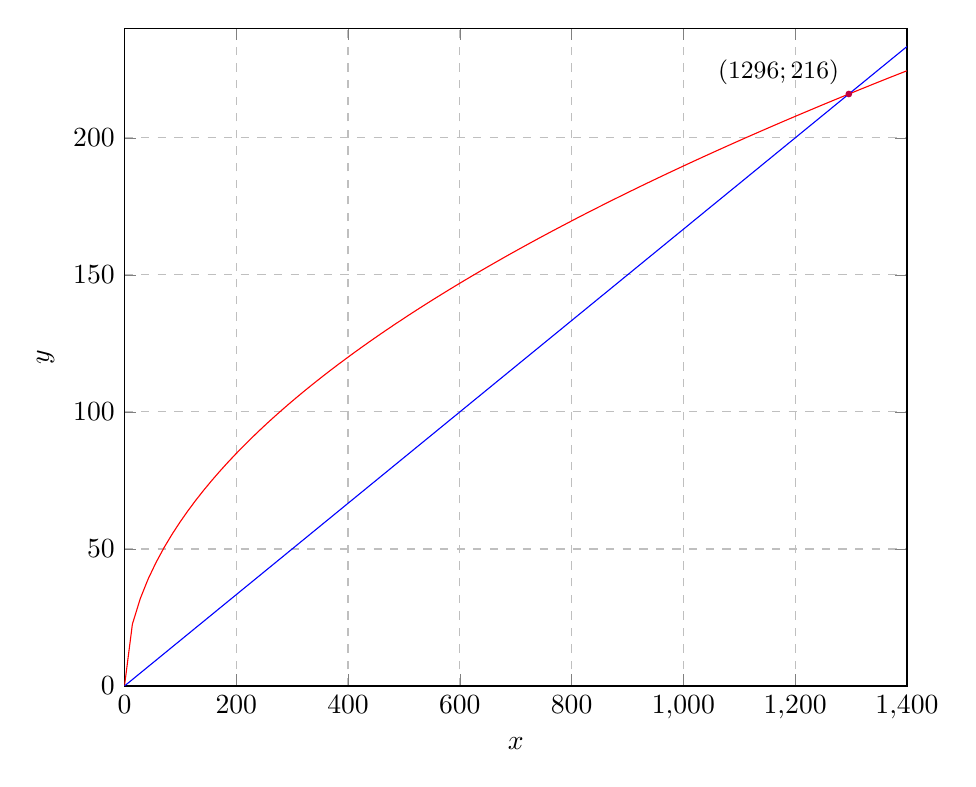
\begin{tikzpicture}
    \begin{axis}[
        width=0.95\textwidth,
        xlabel = \(x\),
        ylabel = \(y\),
        xmin = 0, xmax = 1400,
        ymin = 0, ymax = 240,
        grid = major,
        grid style = dashed,
      ]

      \addplot[
        domain=0:1400,
        samples=100,
        color=red,
      ]{6 * x^(1/2)};

      \addplot[
        domain=0:1400,
        samples=100,
        color=blue,
      ]{x / 6};

      \addplot[
        only marks,
        mark=*,
        mark size=1pt,
        color=purple,
      ] coordinates {(1296, 216)};
      \node[above left] at (axis cs:1296,216) {\small $(1296; 216)$};
    \end{axis}
  \end{tikzpicture}
\end{center}
